\section{Extract Particles}
 \begin{figure}[H]
  \centering
  \captionsetup{width=.8\linewidth} 
  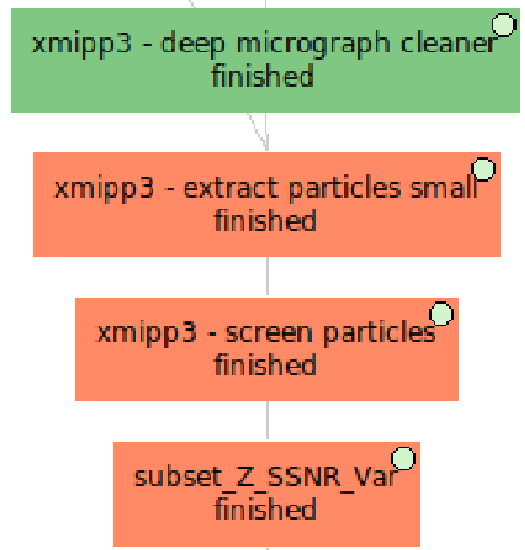
\includegraphics[width=0.45\textwidth]
  {{images/workflow_4_a.pdf}}
  \caption{Extract particles workflow (Orange color).}
  \label{fig:workflow_4_a}
  \end{figure}
Once we have a set of coordinates, we can proceed to extract particles with \ttt{Xmipp} protocol \scommand{xmipp3-extract particles} (\ffigure{fig:xmipp_extract_particles}). This protocol allows to extract, normalize and correct the CTF phases of the selected particles. As input, this protocol requires the set of coordinates and the consensus CTF values obtained in previous steps, and a downsampling factor. To save computing resources, include in the input the desired reduced size of the particles. In this particular case, 74 pixels.

\begin{figure}[H]
  \centering
  \captionsetup{width=.8\linewidth} 
  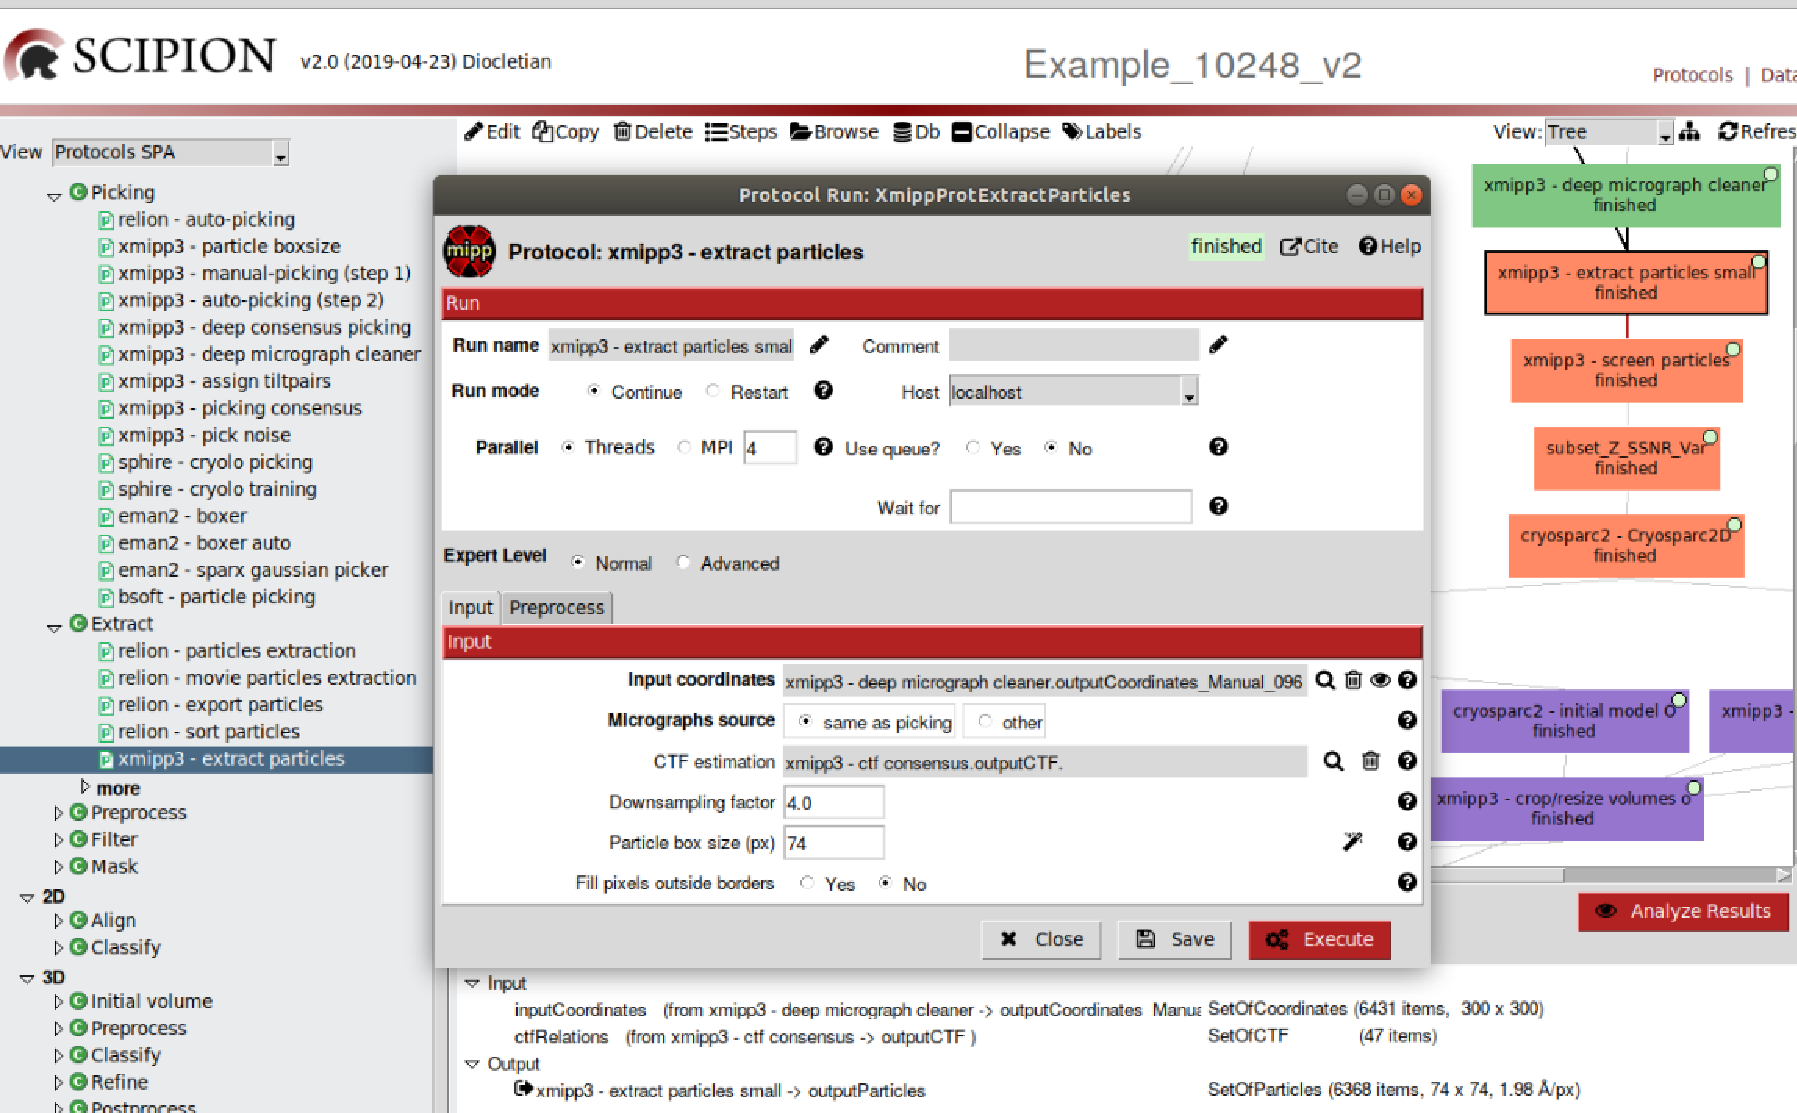
\includegraphics[width=0.95\textwidth]
  {images/xmipp_extract_particles.pdf}
  \caption{Filling in the protocol \scommand{xmipp3-extract particles}.}
  \label{fig:xmipp_extract_particles}
  \end{figure}
  
  The form tap \ttt{Preprocess} gives you additional options:
  \begin{itemize}
   \item \ttt{Invert contrast}: Option \ttt{Yes} means that bright regions become dark and the other way around.
   \item \ttt{Phase flipping}: Option \ttt{Yes} means that the protocol corrects \ttt{CTF} phases of the particles.
   \item \ttt{Normalize}: Option \ttt{Yes} (recommended) means that the particles are normalized with zero mean and one as standard deviation for background pixels.
  \end{itemize}

  As output, the protocol generates a new set of 6,368 particles after discarding other 63 particles. The extracted particles harbor the smaller selected size and 4 times the initial sampling rate. The images of the normalized extracted particles can be seen pressing \scommand{Analyze Results}. By default, particles displayed in gallery mode can be sorted by \ttt{Zscore}. To visualize the score associated to each particle, switch the table view by pressing the top left button. If you want to remove any of the particles showing lower score values, select them, press the mouse right button and choose \ttt{Disable}. A new subset of particles can be created by clicking on \ttt{Particles} red button. 
  
  \subsection*{Particle cleaning}
  
  Additional cleaning steps of bad particles can be performed with other screening protocols such as \scommand{xmipp3-screen particles} (\ffigure{fig:xmipp_screen_particles}). The protocol input is the subset of particles previously generated. Three different criteria for rejection can be selected, \ttt{Zscore}, \ttt{SSNR} and \ttt{Variance}. Zscore assesses the similarity of each particle with the average. SSNR evaluates the signal to noise ration in the Fourier space. The variance is assessed for each particle in the context of particles where that particle was picked. In this particular case, we are not going to set any of the mentioned params (Zscore, SSNR and Variance). Instead, selection will be performed after visualizing the plots of those statistics. 
  
  \begin{figure}[H]
  \centering
  \captionsetup{width=.8\linewidth} 
  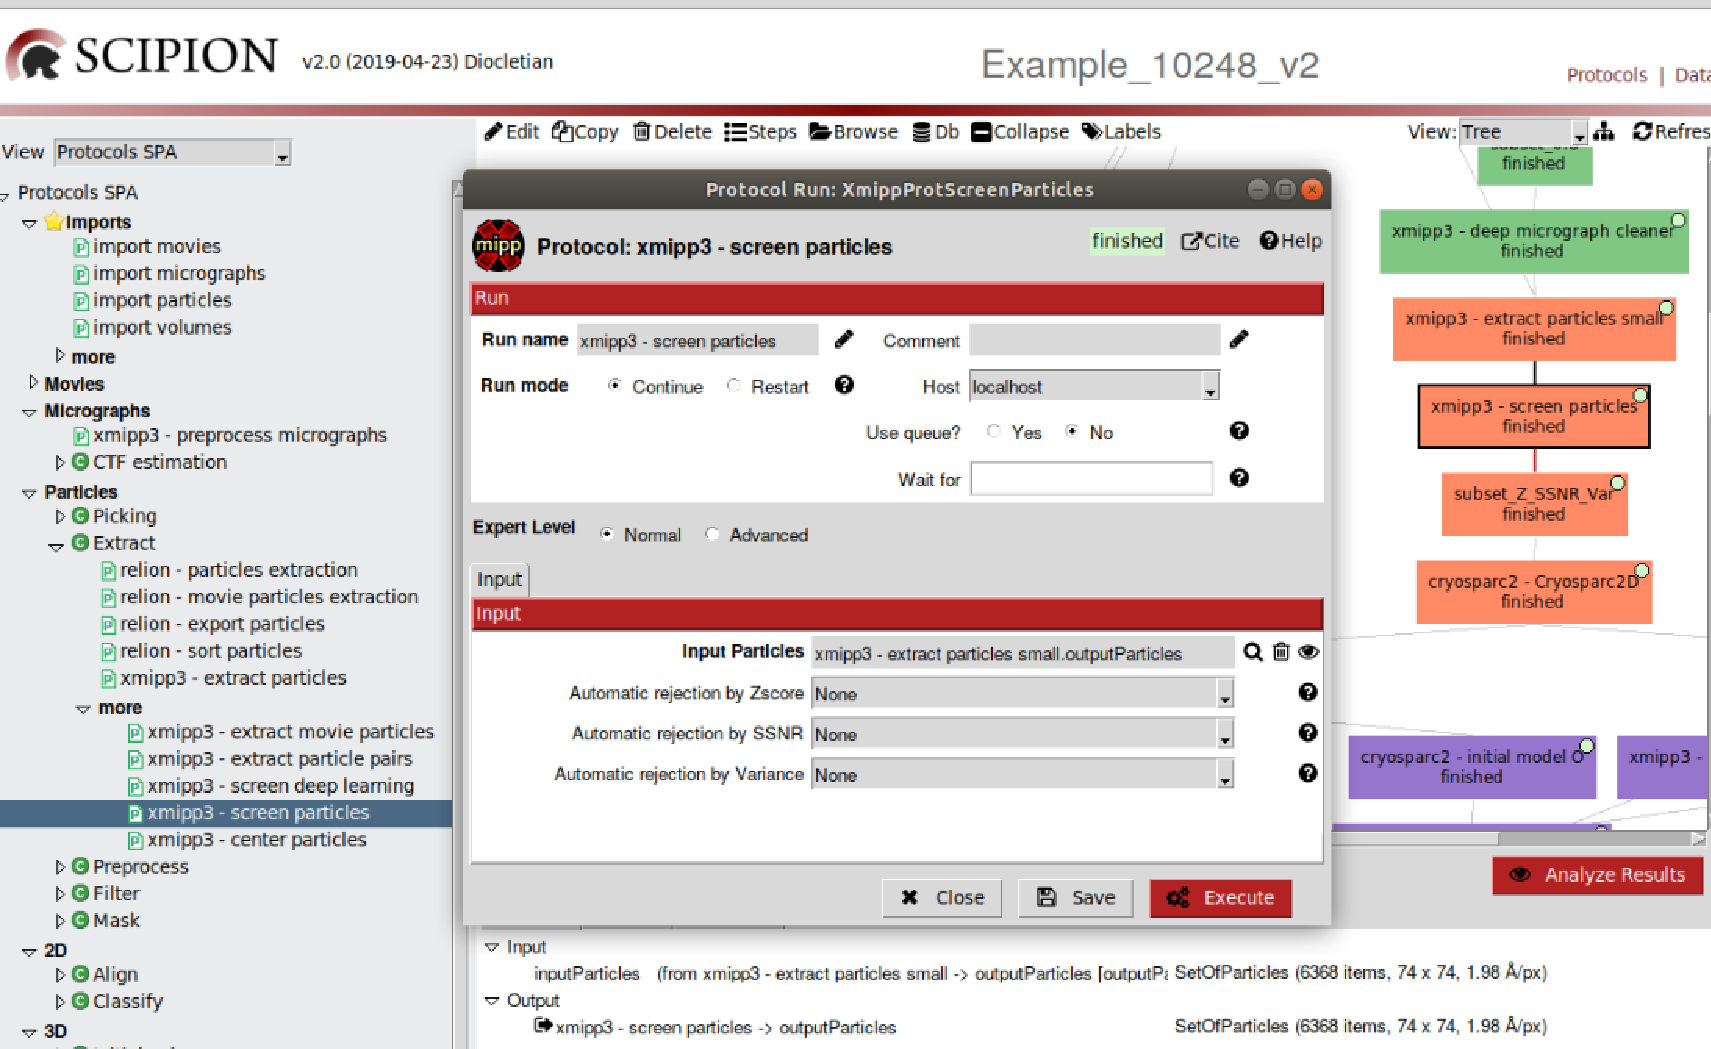
\includegraphics[width=0.95\textwidth]
  {images/xmipp_screen_particles.pdf}
  \caption{Completing the protocol \scommand{xmipp3-screen particles}.}
  \label{fig:xmipp_screen_particles}
  \end{figure}
  
  After executing the protocol without discarding any particles, we press \scommand{Analyze Results}. The plot of \ttt{Zcore} and the \ttt{Variance} histogram will be open, together with the table of particles. According to the \ttt{Zcore} plot, we discard particles with \ttt{Zcore} value higher than 3.0. According to the \ttt{Variance} histogram, we reject particles with \ttt{Variance} higher than 1.21. We can also visualize the histogram of \ttt{\_xmipp\_cumulativeSSNR}. According to this histogram, particles with \ttt{SSNR} values lower than 2.5 and higher than 5 will be discarded. The new subset of ``cleaned'' particles  obtained according those specific criteria (\ttt{subset\_Z\_SSNR\_Var}) contains 5,913 particles after discarding 455 of them (7.1\%), that can be observed pressing \scommand{Analyze Results}. This new subset of selected particles is considered reliable for further image processing.
